\label{sec:task-par}

Data based workflow engines exploit task-parallelism by partitioning the data and generating stages of independent tasks.
These stages then ordered and implement data dependencies by shuffling, aggregating or coupling intermediate results.
The MapReduce~\cite{dean2004mapreduce} abstraction, along with its implementations, popularized this method of processing.

Spark~\cite{zaharia2010spark} and Dask~\cite{rocklin2015dask} are two Big Data frameworks.
Both provide MapReduce abstractions and are optimized for parallel processing of large data volumes, interactive analytics and machine learning.
Their runtime engines can automatically partition data, generate parallel tasks, and execute them on a cluster.
In addition, Spark offers in-memory capabilities allowing caching data that are read multiple times, making it suited for interactive analytics and iterative machine learning algorithms.
Dask also provides a MapReduce API (Dask Bags).
Furthermore, Dask's API is more versatile, allowing custom workflows and parallel vector/matrix computations.

\section{Molecular Dynamics (MD) Data Analysis}
%\label{ssec:use_cases}
Some commonly used algorithms for analyzing MD trajectories are Root Mean Square Deviation (RMSD), Pairwise Distances (PD), and Sub-setting~\cite{mura2014biomolecules}.
Two more advanced algorithms are Path Similarity Analysis (PSA)~\cite{seyler2015path} and Leaflet Identification~\cite{michaud2011mdanalysis}.
RMSD is used to identify the deviation of atom positions between frames.
PD and PSA methods calculate distances based on different metrics either between atoms or trajectories.
Sub-setting methods are used to isolate parts of interest of MD simulation.
Leaflet Identification provides information about groups of lipids by identifying the lipid leaflets in a lipid bilayer.
All these methods, in some way, read and process the whole physical system generated via simulations.
The analysis reduces the data to either a number or a matrix.

We discuss two of these methods, a Path Similarity Analysis (PSA) algorithm using the Hausdorff distance and a Leaflet Identification method, and their implementations in MDAnalysis~\cite{michaud2011mdanalysis,gowers2016mdanalysis}.
Section~\ref{ssec:mda} discusses the reasons for selecting these two algorithms in more detail.
%In addition, we implemented the PSA algorithm using CPPTraj~\cite{roe2013ptraj}.
%Furthermore, we explore the applications' Ogres Facets and Views~\cite{fox2014towards}, which provide a more systematic characterization.

%Big Data Ogres~\cite{fox2014towards} are organized into four classes, called \emph{views}.
%The possible features of a view are called \emph{facets}.
%A combination of facets from all views defines an Ogre.
%The Views are: 
%\begin{inparaenum}[1)]
%    \item execution - describes aspects, such as I/O, memory, compute ratios, whether computations are iterative, and the 5 V's of Big Data (Volume, Velocity, Value, Variety and Veracity),
%    \item data source \& style - discusses input data collection, storage and access,
%    \item processing - describes algorithms and kernels used for computation, and
%    \item problem architecture - describes the application architecture.
%\end{inparaenum}


\subsection{Applications and Algorithms: MDAnalysis}
\label{ssec:mda}
MDAnalysis is a Python library~\cite{michaud2011mdanalysis,gowers2016mdanalysis} that provides a comprehensive environment for filtering, transforming and analyzing MD trajectories in all commonly used file formats.
It provides a common object-oriented API to trajectory data and leverages existing libraries in the scientific Python software stack, such as NumPy~\cite{numpy} and Scipy~\cite{scipy}.

\subsubsection*{Path Similarity Analysis (PSA): Hausdorff Distance}Path Similarity Analysis (PSA)~\cite{seyler2015path} is used to quantify the similarity between trajectories considering their full atomic detail.
The basic idea is to compute pair-wise distances (for instance, using the Hausdorff metric~\cite{huttenlocher1993comparing}) between members of an ensemble of trajectories and cluster the trajectories based on their distance matrix.

Each trajectory is represented as a two dimensional array.
The first dimension corresponds to time frames of the trajectory, the second to the $N$ atom positions, in 3-dimensional space.

\begin{algorithm}[t]
    \scriptsize
    \caption{Path Similarity Algorithm: Hausdorff Distance}
    \label{alg:hausdorff}
    \begin{algorithmic}[1]
        \Procedure{HausdorffDistance}{$T_1$,$T_2$}\Comment{$T_1$ and $T_2$ are a set of 
            3D points}
        \State \texttt{List $D_1$,$D_2$}
        \For{$\forall frame_1$ in $T_1$}
        \For{$\forall frame_2$ in $T_2$}
        \State \texttt{Append in $D_1$ $d_{RMS}$($frame_1$, $frame_2$)}
        \EndFor
        \State \texttt{$D_{t_1}$ append $min(D_1)$}
        \EndFor
        \For{$\forall frame_2$ in $T_2$}
        \For{$\forall frame_1$ in $T_1$}
        \State \texttt{Append in $D_2$ $d_{RMS}$($frame_2$, $frame_1$)}
        \EndFor
        \State\texttt{$D_{t_2}$ append $min(D_2)$}
        \EndFor
        \State \textbf{return} $max\Big(max(D_{t_1}),max(D_{t_2})\Big)$
        \EndProcedure
        \\        
        \Procedure{PSA}{$Traj$}\Comment{$Traj$ is a set of trajectories}
        \For{$\forall T_1$ in $Traj$}
        \For{$\forall T_2$ in $Traj$}
        \State \texttt{ $D_{( T_1,T_2 )}$=HausdorffDistance$\Big( T_1,T_2 \Big)$} 
        \EndFor
        \EndFor
        \State \Return $D$
        \EndProcedure
    \end{algorithmic}
\end{algorithm}

Algorithm~\ref{alg:hausdorff} describes the PSA algorithm with the Hausdorff metric over multiple trajectories.
We apply a 2-dimensional data partitioning over the output matrix to parallelize, shown in algorithm~\ref{alg:partition}.
Our Hausdorff metric calculation is based on a naive algorithm.
Recently, an algorithm was introduced that uses early break to speedup execution~\cite{taha2015efficient}, although we are not aware of a parallel implementation of this algorithm.

\begin{algorithm}[t]
    \scriptsize
    \caption{Two Dimensional Partitioning}
    \label{alg:partition}
    \begin{algorithmic}[1]
        \State Initially, there are $N^2$ distances, where $N$ is the number of trajectories.
        Each distance defines a computation task.
        \State Map the initial set to a smaller set with $k=N/n_1$ elements, where $n_1$ is a divisor of $N$, by grouping $n_1$ by $n_1$ elements together.
        \State Execute over the new set with $k^2$ tasks.
        Each task is the comparisons between $n_1$ and $n_1$  elements of the initial set.
        They are executed serially.
    \end{algorithmic}
\end{algorithm}

The algorithm is embarrassingly parallel and uses linear algebra kernels for calculations.
It has complexity $O(n^2)$ (problem architecture \& processing views).
Input data volume is medium to large while the output is small.
Specific execution environments, such as HPC nodes, and Python arithmetic libraries, e.g., NumPy, are used (execution view).
Input data are produced by HPC simulations, and are stored on HPC storage systems, such as parallel filesystem like Lustre (data source \& style view).

Embarrassingly parallel algorithms are good candidates to utilize task parallelization.
The data are partitioned to independent parts and each part is assigned to a task.
These tasks can then execute as a bag of tasks.
As a result, they are ideally suited for task-management and MapReduce APIs.
They can be expressed as a bag of tasks using a task management API or a map-only application in a MapReduce-style API.
All three selected frameworks support the execution of bag of tasks, with RADICAL~-Pilot and Dask offering specific abstractions (as discussed in \S~\ref{ssec:frameworks}).

\subsubsection*{Leaflet Finder}Algorithm~\ref{alg:leafletfinder} describes the Leaflet Finder (LF) algorithm as presented in Ref.~\cite{michaud2011mdanalysis}.
LF assigns particles to one of two curved but locally approximately parallel sheets, provided that the inter-particle distance is smaller than the distance between sheets.
In biomolecular simulations of lipid membranes, consisting of a double layer of lipid molecules, LF is used to identify the lipids in the outer and inner leaflets (sheets).
The algorithm consists of two stages:
\begin{inparaenum}[a)]
    \item construction of a graph connecting particles based on threshold distance (cutoff), and
    \item computing the connected components of the graph, determining the lipids located on the outer and inner leaflets.
\end{inparaenum}

\begin{algorithm}[t]
    \scriptsize
    \caption{Leaflet Finder Algorithm}
    \label{alg:leafletfinder}
    \begin{algorithmic}[1]
        \Procedure{LeafletFinder}{$Atoms,Cutoff$}
        \Comment{$Atoms$ is a set of 3D points that represent the position of atoms in space. $Cutoff$ is an Integer Number}
        \State \texttt{Graph G =$(V=Atoms,E=\emptyset)$}
        \For{$\forall atom$ in $Atoms$}
        \State \texttt{$N = [a\in V: d(a,atom)\le Cutoff]$}
        \State \texttt{Add edges $[(atoms,a): a \in N]$ in G}
        \EndFor
        \State \texttt{C = ConnectedComponents(G)}
        \State \Return C
        \EndProcedure
    \end{algorithmic}
\end{algorithm}

The application stages have different complexities.
The first stage identifies neighboring atoms.
There are different implementation alternatives: 
\begin{inparaenum}[i)]
    \item computing the distance between all atoms ($O(n^2)$);
    \item utilizing a tree-based nearest neighbor (Construction: $O(n\log n)$, 
    Query: $O(\log n)$).
\end{inparaenum}
In both alternatives the input data volume is medium size and the output is smaller than the input.
The complexity of connected components is: $O(|V|+|E|)$ ($V$: Vertices, $E$: Edges), i.\,e. it greatly depends on the characteristics of the graph.

The application typically uses HPC nodes as the execution environment, and NumPy arrays (execution view).
It uses matrices to represent the physical system and the distance matrix.
The output data representation is a graph.
Leaflet Finder can be efficiently implemented using the MapReduce abstraction (problem architecture view).
It uses graph algorithms and linear algebra kernels (processing view facets).
The data source \& style view facets are the same as the PSA algorithm.

Leaflet Finder is more complex as it requires two stages.
It is possible to implement Leaflet Finder with a simple task-management API, although the MapReduce programming model allows more efficient implementation with a \texttt{map} for computing and filtering distances and a \texttt{reduce} for finding the components.
The shuffling required between map and reduce is medium as the number of edges is a fraction of the input data.
Spark and Dask natively support MapReduce and implementinf the Leaflet Finder algorithm is relatively straightforward.
RADICAL-Pilot, on the other hand, does not support natively MapReduce.
As a result, it is required by the application developer to define the data shuffling between the \emph{map} and \emph{reduce} phase of the algorithm.

%\subsubsection{CPPTraj}
%CPPTraj~\cite{roe2013ptraj,roe2018parallelization} is a C++ MD trajectory analysis tool.
%It is parallelized via MPI and OpenMP.
%CPPtraj reads in parallel frames from a single trajectory file or ensemble members of the same trajectory from different files.
%The frames are equally distributed to the MPI processes.
%Computational intensive algorithms are further parallelized using OpenMP.
%It requires at least one MPI process per ensemble member, where each member is a single trajectory file.


\subsection{Current Solutions for Parallel MD Data Analysis}
\label{ssec:related_work}
MD analysis algorithms were until recently executed serially and parallelization was not straightforward.
During the last years several frameworks emerged providing parallel algorithms for analyzing MD trajectories.
Some of those frameworks are CPPTraj~\cite{roe2013ptraj,roe2018parallelization}, HiMach~\cite{tiankai2008scalable}, PMDA~\cite{fan2019pmda}, Pteros 2.0~\cite{yesylevskyy2015pteros} and nMoldyn-3~\cite{hinsen2012nmoldyn}.
%We compare these frameworks with our approach over the parallelization techniques used.

Several different techniques are used for parallelizing these algorithms.
CPPTraj~\cite{roe2018parallelization} utilizes MPI and OpenMP to exeucte large scale analysis on HPC.
OpenMP is also utilized by Pteros~\cite{yesylevskyy2015pteros} to parallelize the compute intensive parts of the analysis.
HiMach~~\cite{tiankai2008scalable} extends Google's MapReduce and defines Map and Reduce methods.
nMoldyn-3~\cite{hinsen2012nmoldyn} parallelizes the execution through a Master Worker architecture.
The master defines analysis tasks, submits them to a task manager, which then are executed by the worker process.

%HiMach~\cite{tiankai2008scalable} was developed by D. E. Shaw Research group to provide a parallel analysis framework for MD simulations, and extends Google's MapReduce.
%HiMach API defines trajectories, does per frame data acquisition (Map) and cross-frame analysis (Reduce).
%HiMach's runtime is responsible to parallelize and distribute Map and Reduce phases to resources.
%Data transfers are done through a communication protocol created specifically for HiMach.

%Pteros-2.0~\cite{yesylevskyy2015pteros} is a open-source library that is used for modeling and analyzing MD trajectories, providing a plugin for each supported algorithm.
%The execution is done by a user defined driver application, which setups trajectory  I/O and frame dispatch for analysis.
%It offers a C++ and Python API.
%Pteros 2.0 parallelizes computational intensive algorithms via OpenMP and Multithreading.
%As a result, it is bounded to execute on a single node, making any analysis execution highly dependent on memory size.
%Through RADICAL-Pilot, Spark and Dask, we avoided recompiling every time there is a change to the underlying resource, ensuring the application's execution.

%MDTraj~\cite{mcgibbon2015mdtraj} is a Python package for analyzing MD trajectories.
%It links MD data and Python statistical and visualization software.
%MDTraj proposes parallelizing the execution by using the parallel package of IPython as a wrapper along with an out-of-core trajectory reading method.
%Our approach allows data parallelization on any level of the execution, not only in data read.

%nMoldyn-3~\cite{hinsen2012nmoldyn} parallelizes the execution through a Master Worker architecture.
%The master defines analysis tasks, submits them to a task manager, which then are executed by the worker process.
%In addition, it provides adaptability, allowing on-the-fly addition of resources, and execution fault tolerance when worker processes disconnect.

A common denominator of most approaches is that they do not use general purpose frameworks for parallelizing the execution.
Although, they are optimized to get as much performance as possible from the environments they are developed for, their portability is limited.
CPPTraj~\cite{roe2018parallelization} and Pteros~\cite{yesylevskyy2015pteros}, for example, are highly dependent on the underlying low level libraries of the resource they use.
HiMach~\cite{tiankai2008scalable} is build specifically for the Antons Supercomputer.

In contrast, our approach and PMDA~\cite{fan2019pmda} utilize more general purpose frameworks for parallelization.
Specifically, PMDA utilizes Dask to parallelize MD Trajectory analysis.
The frameworks used provide higher level abstractions, e.g machine learning, so any  integration with other data analysis methods can be fast and easier.
In addition, resource acquisition and management is done transparently.

\section{Task-Parallel Frameworks: RADICAL-Pilot, Spark, Dask}
\label{ssec:frameworks}
The landscape of frameworks for data-intensive applications is manifold~\cite{jha2014tale,kamburugamuve2017anatomy} and has been extensively studied in the context of scientific~\cite{jha2017introducing} applications.
In this section, we discuss the suitability of frameworks such as Spark~\cite{zaharia2010spark}, Dask~\cite{rocklin2015dask} and RADICAL~-Pilot~\cite{merzky2019using}, for MD data analytics.

\subsection{Background}
%MapReduce~\cite{dean2004mapreduce} and its open source Hadoop implementation combined a simple functional API with a powerful distributed computing engine that exploits data locality to allow optimized I/O performance.
%However, MapReduce is inefficient for interactive workloads and iterative machine learning algorithms~\cite{zaharia2010spark,ekanayake2010twister}.
Spark and Dask provide rich APIs, caching and other capabilities critical for analytics applications.
Spark is considered the standard solution for iterative data-parallel applications.
Dask is quickly gaining support in the scientific community, since it offers a fully python environment.
RADICAL~-Pilot is a Pilot-Job framework~\cite{luckow2012pstar} that supports task-level parallelism on HPC resources and adds a parallelization level on top of HPC MPI-based applications.
%RADICAL~-Pilot is a Pilot-Job framework~\cite{luckow2012pstar} that supports task-level parallelism on HPC resources.
%It successfully adds a parallelization level on top of HPC MPI-based applications.

As described in~\cite{jha2014tale}, these frameworks typically comprise of distinct layers, e.\,g.,cluster scheduler access, framework-level scheduling, and higher-level abstractions.
On top of low-level resource management capabilities various higher-level abstractions can be provided, e.\,g., MapReduce-inspired APIs.
These then provide the foundation for analytics abstractions, such as Dataframes, Datasets and Arrays.
Figure~\ref{fig:figures_bigdata_framework_stack} visualizes the different components of RADICAL~-Pilot, Spark and Dask.
The following describes each framework in detail.

\begin{figure}[ht]
    \centering
    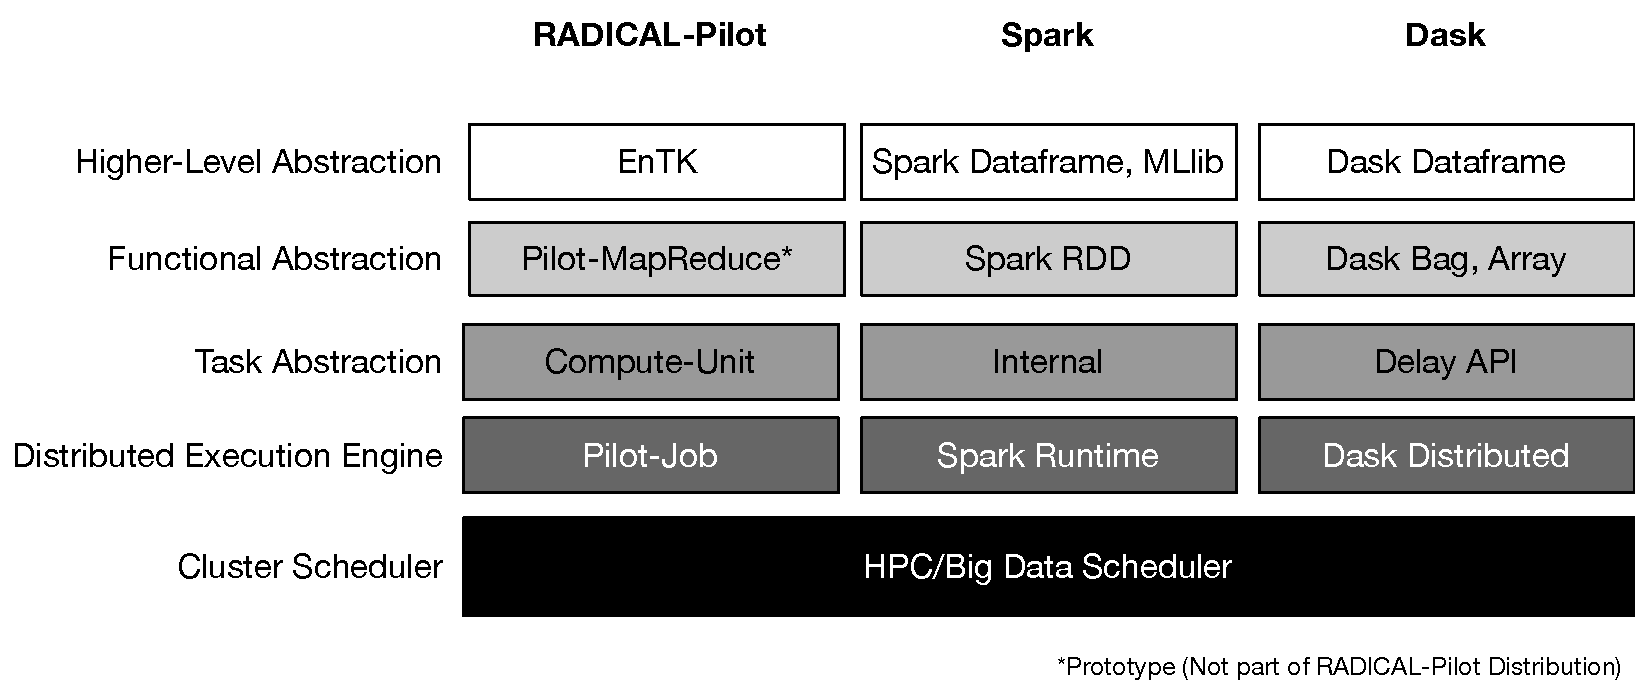
\includegraphics[width=.95\textwidth]{figures/data_analytics_hpc/task_par/bigdata_framework_stack.pdf}
    \caption{Architecture of RADICAL~-Pilot, Spark and Dask.}
    %\caption{\textbf{Architecture of RADICAL~-Pilot, Spark and Dask:}
    %The frameworks share common architectural components for managing cluster resource, and tasks.
    %Spark, Dask offer several high-level abstractions inspired by MapReduce.}
    \label{fig:figures_bigdata_framework_stack}
\end{figure}

\subsubsection*{RADICAL-Pilot}
%RADICAL~-Pilot~\cite{merzky2019using} is a Pilot system that implements the pilot paradigm as outlined in Ref.~\cite{turilli2018comprehensive}.
%RADICAL~-Pilot (RP) is implemented in Python and provides a well defined API and usage modes.
%Although RP is vehicle for research in scalable computing, it also supports production grade science.
%Currently, it is being used by applications drawn from diverse domains, ranging from earth and biomolecular sciences to high-energy physics.
%RP can be used as a runtime system by workflow or workload management systems~\cite{turilli2019middleware,treikalis2016repex,balasubramanian2018harnessing,dakka2018high,turilli2017evaluating}.
%In 2017, RP was used to support more than 100M core-hours on US DOE, NSF resources (BlueWaters and XSEDE), and European supercomputers (Archer and SuperMUC).

As discussed in \S~\ref{sec:pilot-data-hadoop}, RADICAL~-Pilot allows concurrent task execution on HPC resources.
The user defines a set of Compute~-Units (CU)~- the abstraction that defines a task along with its dependencies - which are submitted to RADICAL~-Pilot.
RADICAL~-Pilot schedules these CUs to be executed under the acquired resources.
It uses the existing environment of the resource to execute tasks.
Any data communication between tasks is done via an underlying shared filesystem, e.g., Lustre.
Task execution coordination and communication is done through a database (MongoDB).

%RADICAL~-Pilot's learning curve can be quite steep at the beginning, at least until the user becomes familiar with the concept and usability of Pilots and CUs.
%Once the user is comfortable with RADICAL~-Pilot's API, she can easily develop new algorithms.

\subsubsection*{Spark}
Spark~\cite{zaharia2010spark} extends MapReduce~\cite{dean2004mapreduce} providing a rich set of operations on top of the Resilient Distributed Dataset (RDD) abstraction~\cite{zaharia2012resilient}.
RDDs are cached in-memory making Spark well suitable for iterative applications that need to cache a set of data across multiple stages.
PySpark provides a Python API to Spark.

A Spark job is compiled of multiple stages; a stage is a set of parallel tasks executed without communicating (e.\,g., \texttt{map}) and an action (e.\,g., \texttt{reduce}).
Each action defines new stage.
The \texttt{DAGScheduler} is responsible for translating the workflow specified via RDD transformations and actions to an execution plan.
Spark's distributed execution engine handles the low-level details of task execution.
The execution of a Spark job is triggered by actions.
Spark can read data from different sources, such as HDFS, blob storage, parallel and local filesystems.
While Spark caches loaded data in memory, it offloads to disk when an executor does not have enough free memory to hold all the data of its partition.
Persisted RDDs remain in memory, unless specified to use the disk either complementary or as a single target.
In addition, Spark writes to disk data that are used in a shuffle.
As a result, it allows quick access to those data when transmitted to an executor.
Finally, Spark provides a set of actions that write text files, Hadoop sequence files or object files to local filesystems, HDFS or any filesystem that supports Hadoop.
In addition, Spark supports higher-level data abstractions for processing structured data, such as dataframes, Spark-SQL, datasets, and data streams.

\subsubsection*{Dask}
Dask~\cite{rocklin2015dask} provides a Python-based parallel computing library, which is designed to parallelize native Python code written for NumPy and Pandas.
In contrast to Spark, Dask also provides a lower-level task API (\texttt{delayed} API) that allows users to construct arbitrary workflow graphs.
Being written in Python, it does not require to translate data 
types from one language to another like PySpark, which moves data between Python's interpreter and Java/Scala.

In addition to the low-level task API, Dask offers three higher-level abstractions: Bags, Arrays and Dataframes.
Dask Arrays are a collection of NumPy arrays organized as a grid.
Dask Bags are similar to Spark RDDs and are used to analyze semi-structured data, like JSON files.
Dask Dataframe is a distributed collection of Pandas dataframes that can be analyzed in parallel.

Furthermore, Dask offers three schedulers: multithreading, multiprocessing and distributed.
The multithreaded and multiprocessing schedulers can be used only on a single node and the parallel execution is done via threads and processes respectively.
The distributed scheduler creates a cluster with a scheduling process and multiple worker processes.
A client process creates and communicates a DAG to the scheduler.
The scheduler assigns tasks to workers.

Dask's learning curve cannot be considered steep.
Its API is well defined and documented.
In addition, familiarity with Spark or MapReduce helps to minimize the learning curve even further.
As a result, implementing MD analysis algorithms on Dask did not require significant engineering time.
In addition, setting up a Dask cluster on a set of resources was relatively straightforward, since it provides all the binaries, e.g. \texttt(dask-ssh).

%\subsubsection*{RADICAL-Pilot}
%RADICAL~-Pilot~\cite{merzky2019using} is a Pilot system that implements the pilot paradigm as outlined in Ref.~\cite{turilli2018comprehensive}.
%RADICAL~-Pilot (RP) is implemented in Python and provides a well defined API and usage modes.
%Although RP is vehicle for research in scalable computing, it also supports production grade science.
%Currently, it is being used by applications drawn from diverse domains, ranging from earth and biomolecular sciences to high-energy physics.
%RP can be used as a runtime system by workflow or workload management systems~\cite{turilli2019middleware,treikalis2016repex,balasubramanian2018harnessing,dakka2018high,turilli2017evaluating}.
%In 2017, RP was used to support more than 100M core-hours on US DOE, NSF resources (BlueWaters and XSEDE), and European supercomputers (Archer and SuperMUC).

%RADICAL~-Pilot allows concurrent task execution on HPC resources.
%The user defines a set of Compute~-Units (CU)~- the abstraction that defines a task along with its dependencies - which are submitted to RADICAL~-Pilot.
%RADICAL~-Pilot schedules these CUs to be executed under the acquired resources.
%It uses the existing environment of the resource to execute tasks.
%Any data communication between tasks is done via an underlying shared filesystem, e.g., Lustre.
%Task execution coordination and communication is done through a database (MongoDB).

%RADICAL~-Pilot's learning curve can be quite steep at the beginning, at least until the user becomes familiar with the concept and usability of Pilots and CUs.
%Once the user is comfortable with RADICAL~-Pilot's API, she can easily develop new algorithms.

\subsection{Comparison}
\begin{table}[t]
    \begin{tabular}{@{}p{2.75cm}|p{3.25cm}p{3.25cm}p{3.25cm}@{}}
        \toprule
        &\textbf{RADICAL-Pilot} &
        \textbf{Spark} &
        \textbf{Dask} \\
        \midrule
        % row 1
        Languages &
        Python &
        Java, Scala, Python, R &
        Python\\
        % Row 2
        Task &
        Task &
        Map-Task &
        Delayed\\
        % row 3
        Abstraction &
        &
        & \\
        % row 4
        Functional Abstraction  &
        - &
        RDD API &
        Bag\\
        % row 5        
        Higher-Level Abstractions &
        EnTK~\cite{balasubramanian2018harnessing} &
        Dataframe, ML Pipeline, MLlib~\cite{meng2016mllib} &
        Dataframe, Arrays for block computations\\
        % row 6
        Resource Management &
        Pilot-Job &
        Spark Execution Engines &
        Dask Distributed Scheduler\\
        % row 7
        Scheduler    &
        Individual Tasks &
        Stage-oriented DAG &
        DAG\\
        % row 8        
        Shuffle      &
        -       &
        hash/sort-based shuffle &
        hash/sort-based shuffle\\
        % row 8
        Limitations &
        no shuffle, filesystem-based communication  &
        high overheads for Python tasks (serialization)   &
        Dask Array can not deal with dynamic output shapes\\
        \bottomrule
    \end{tabular}
    \caption{Task-parallel Frameworks Comparison.\label{tab:frameworks}}
    %\caption{\textbf{Task-parallel Frameworks Comparison:} Dask and Spark are designed for data-related task, while RADICAL~-Pilot focuses on compute-intensive tasks.\label{tab:frameworks}}
\end{table}

Table~\ref{tab:frameworks} summarizes the properties of these frameworks with respect to abstractions and runtime provided to create and execute parallel data applications. 

\subsubsection*{API and Abstractions} 
RADICAL~-Pilot provides a low-level API for executing tasks onto resources.
While this API can be used to implement high-level capabilities, e.\,g. MapReduce~\cite{mantha2012pilot}, they are not provided out-of-the box.
Both Spark and Dask provide such capabilities.
Dask's API is generally lower level than Spark's , e.\,g., it allows specifying arbitrary task graphs.
Although, data partition size is automatically decided, in many cases it is necessary to tune parallelism by specifying the number of partitions.

Another important aspect is the availability of high-level abstractions.
High-level tools for RADICAL~-Pilot, such as Ensemble Toolkit~\cite{balasubramanian2018harnessing}, are designed for workflows involving compute-intensive tasks.
Spark and Dask already offer a set of high-level data-oriented abstractions, such as Dataframes.

\subsubsection*{Scheduling}
Both Spark and Dask create a Direct Acyclic Graph (DAG) based on operations over data, which is then executed using their execution engine.
Spark jobs are separated into stages.
When a stage is completed, the scheduler executes the next stage.

Dask's DAGs are represented by a tree where each node is a task.
Leaf tasks do not depend on other task for execution.
Dask tasks are executed when their dependencies are satisfied, starting from leaf tasks.
When a task is reached with unsatisfied dependencies, the scheduler executes the dependent task first.
Dask's scheduler does not rely on synchronization points that Spark's stage-oriented scheduler introduces.
RADICAL~-Pilot does not provide a DAG and requires the execution order and synchronization to be specified by the user.

\subsection{Frameworks Evaluation}
\label{sec:framework_eval}

As data-parallelism often involves a large number of short-running tasks, task throughput is a critical metric to assess the different frameworks.
To evaluate the throughput we use zero workload tasks (\texttt{/bin/hostname}).
We submit an increasing number of such tasks to RADICAL~-Pilot, Spark and Dask and measure the execution time on a single node.

For RADICAL~-Pilot, all tasks were submitted simultaneously. RADICAL~-Pilot's backend database was running on the same node to avoid large communication latencies.
For Spark, we created an RDD with as many partitions as the number of tasks -- each partition is mapped to a task by Spark.
For Dask, we created tasks using \texttt{delayed} functions that were executed by the Distributed scheduler.
We used Wrangler and Comet for this experiment.

\begin{figure}[t]
    \centering
    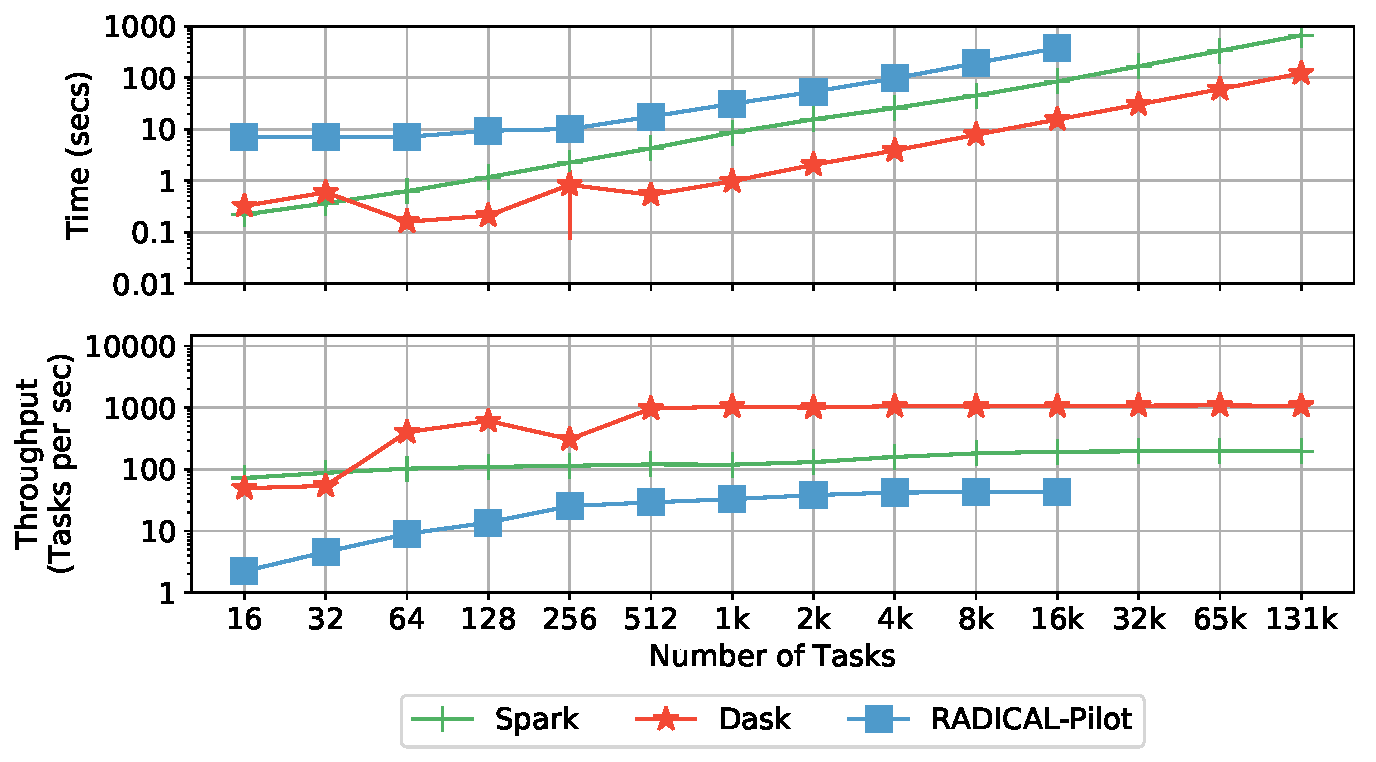
\includegraphics[width=.95\textwidth]{figures/data_analytics_hpc/task_par/dask_spark_rp_wrangler.pdf}
    \caption{Total time to completion and task throughput by framework on a single node for an increasing number of tasks.}
    %\caption{\textbf{Task Throughput by Framework (Single Node):} 
    %    Time/Throughput executing a given number of zero-workload tasks on Wrangler.
    %    Dask performs best; Dask and Spark have very small delays for few tasks.
    %    RADICAL~-Pilot offers the smallest throughput.}
    \label{fig:dask_spark_rp_wrangler}
\end{figure}

Figure~\ref{fig:dask_spark_rp_wrangler} shows the total time to completion and task throughput.
Dask needed the least time to schedule and execute the assigned tasks, followed by Spark and RADICAL~-Pilot.
Dask and Spark quickly reach their maximum throughput, which is sustained as the number of tasks increased.
RADICAL~-Pilot showed the worst throughput and scalability mainly due to some architectural limitations.
It relies on a MongoDB to communicate between Client and Agent, as well as several components that allow RADICAL~-Pilot to move data and introduce delays in the execution of the tasks.
Thus, we were not able to scale RADICAL~-Pilot to 32k or more tasks.

\begin{figure}[t]
    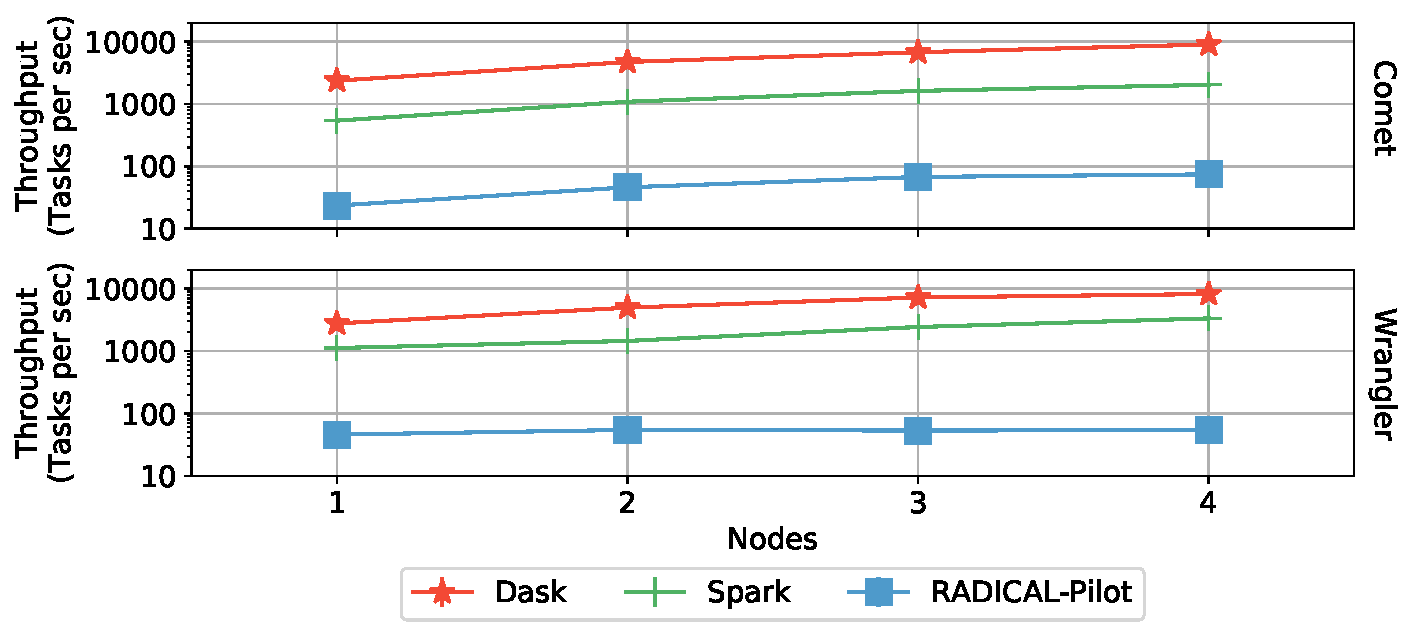
\includegraphics[width=.95\textwidth]{figures/data_analytics_hpc/task_par/daskVSsparkVSRpThroughput.pdf}
    \caption{Task throughput by framewrork for $100k$ tasks on different number of nodes.}
    %\caption{\textbf{Task Throughput by Framework (Multiple Nodes):}
    %    Task throughput for $100k$ zero-workload tasks on different numbers of nodes for each framework. 
    %    Dask has the largest throughput, followed by Spark and RADICAL~-Pilot.}
    \label{fig:RP_Dask_Spark_throughput}
\end{figure}

Figure~\ref{fig:RP_Dask_Spark_throughput} illustrates the throughput when scaling to multiple nodes measured by submitting $100k$ tasks.
Dask's throughput on both resources increases almost linearly to the number of nodes.
Spark's throughput is an order of magnitude lower than Dask's.
RADICAL~-Pilot's throughput plateaus at below $100 task/sec$.
Wrangler and Comet show a comparable performance with Comet slightly outperforming Wrangler.

%\subsubsection*{Suitability for MDAnalysis Algorithms}
%Trajectory analysis methods are often embarrassingly parallel.
%So, they are ideally suited for task management and MapReduce APIs.
%PSA-like methods typically require a single pass over the data and return a set of values that correspond to a relationship between frames or trajectories.
%They can be expressed as a bag of tasks using a task management API or a map-only application in a MapReduce-style API.

%Leaflet Finder is more complex and requires two stages:
%\begin{inparaenum}[a)]
%    \item the edge discovery stage, and
%    \item the connected components stage.
%\end{inparaenum}
%It is possible to implement Leaflet Finder with a simple task-management API, although the MapReduce programming model allows more efficient implementation with a \texttt{map} for computing and filtering distances and a \texttt{reduce} for finding the components.
%The shuffling required between map and reduce is medium as the number of edges is a fraction of the input data.

\section{Task-Parallel MD Trajectory Data Analysis: Implementation \& Characterization}
\label{impl_exp}
In this section, we characterize the performance of RADICAL~-Pilot, Spark and Dask compared to MPI4py.
In section~\ref{sec:framework_eval} we evaluate the task throughput using a synthetic workload.
In sections~\ref{sec:psa} and~\ref{sec:leaflet} we evaluate the performance of two algorithms from MDAnalysis: PSA and Leaflet Finder using different real-world datasets.
We investigate: 
\begin{inparaenum}[1)]
    \item which capabilities and abstractions of the frameworks are needed to efficiently express these algorithms,
    \item what architectural approaches can be used to implement these algorithms with these frameworks, and
    \item the performance trade-offs of these frameworks.
\end{inparaenum}

The experiments were executed on the XSEDE Supercomputers: Comet and Wrangler.
SDSC Comet is a 2.7 PFlop/s cluster with 24\, Haswell cores/node and 128\,GB memory/node (6,400 nodes).
TACC Wrangler has 24\, Haswell hyper-threading enabled cores/node and 128\,GB memory/node (120 nodes).
Experiments were carried using RADICAL~-Pilot and Pilot-Spark (as discusses on \S~\ref{sec:pilot-data-hadoop}) extension, which allows to efficiently manage Spark on HPC resources through a common resource management API.
We utilize a set of custom scripts to start the Dask cluster.
We used RADICAL~-Pilot 0.46.3, Spark 2.2.0, Dask 0.14.1 and Distributed 1.16.3.
The data presented are means over multiple runs; error bars represent the standard deviation of the sample.
We employed up to $10$ nodes in Comet and Wrangler. 

\subsection{Path Similarity Analysis: Hausdorff Distance}
\label{sec:psa}
The PSA algorithm is embarrassingly parallel and can be implemented using simple task-level parallelism or a map only MapReduce application.
The input data, i.\,e. a set of trajectory files, is equally distributed over the cores, generating one task per core.
Each task reads its respective input files in parallel, executes and writes the result to a file.

For RADICAL~-Pilot we define a Compute~-Unit for each task and execute them using a Pilot-Job. 
For Spark, we create an RDD with one partition per task.
The tasks are executed in a \texttt{map} function.
In Dask, the tasks are defined as \texttt{delayed} functions.
In MPI, each task is executed by a process.

The experiments were executed on Comet and Wrangler. 
The dataset used consists of three different atom count trajectories: 
\begin{inparaenum}[1)]
    \item small ($3341$ atoms/frame), 
    \item medium ($6682$ atoms/frame) and 
    \item large ($13364$ atoms/frame).
\end{inparaenum}
We used $102$ frames, and $128$ and $256$ trajectories of each size.

Figure~\ref{fig:HausdorffWrangler} shows the runtime for 128 and 256 trajectories on Wrangler.
Figure~\ref{fig:comet_wrangler_haus} compares the execution times on Comet and Wrangler for $128$ large trajectories.
We see that the frameworks have similar performance on both systems.
Furthermore, we see that Wrangler gives smaller speedup than Comet.
Although, we used the same number of cores, we see that utilizing half the nodes due to hyperthreading results to smaller speedup.

\begin{figure}[t]
    \centering
    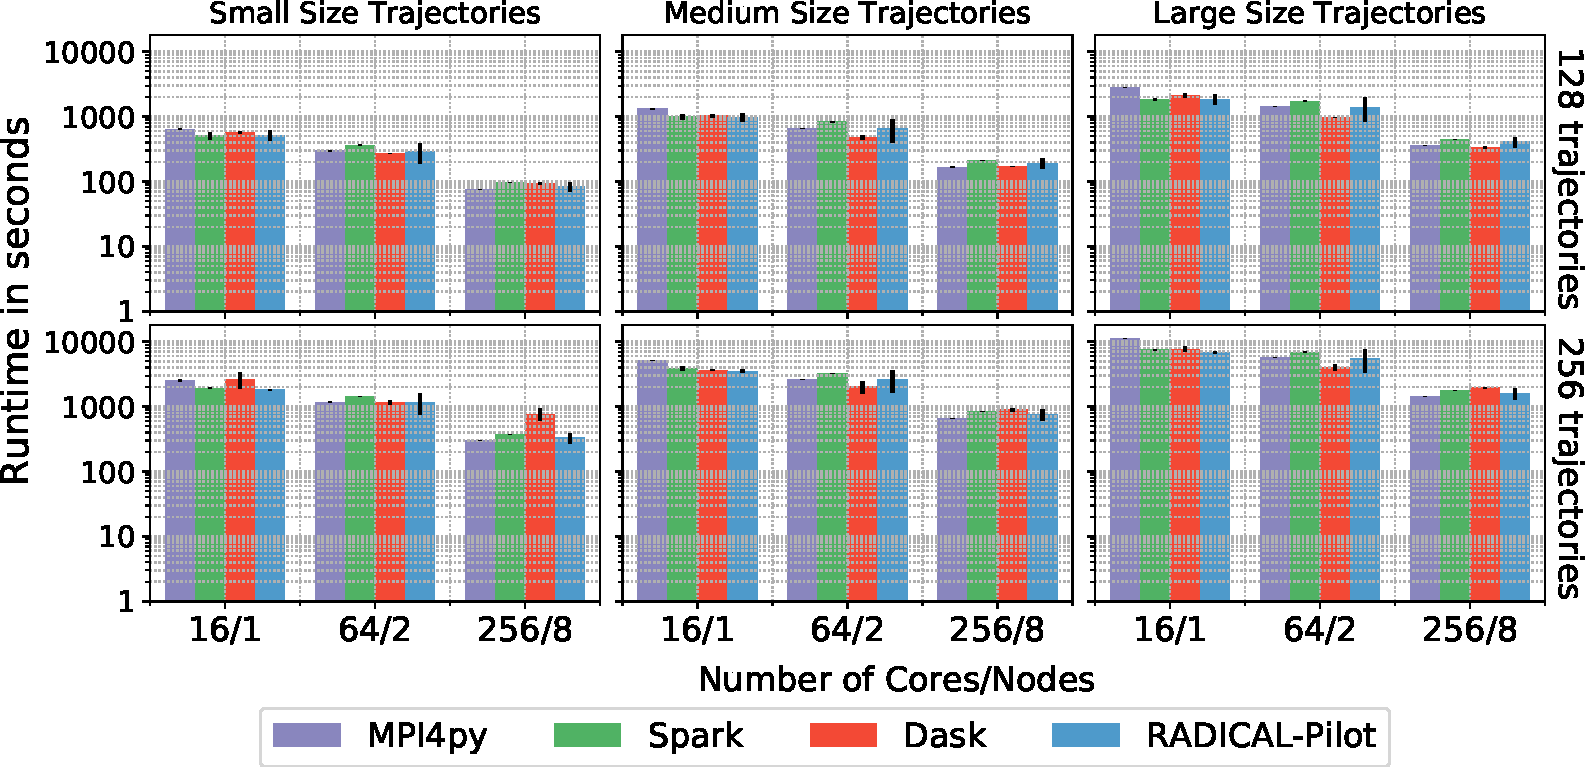
\includegraphics[width=0.95\textwidth]{figures/data_analytics_hpc/task_par/HausdorffSingleFig.pdf}
    \caption{Time to completion of Hausdorff Distance on Wrangler using RADICAL~-Pilot, Spark and Dask over different number of cores, trajectory sizes, and number of trajectories.}
%    \caption{\textbf{Hausdorff Distance on Wrangler using RADICAL~-Pilot, Spark and Dask:}
%            Runtimes over different number of cores, trajectory sizes, and number of trajectories.
%            All frameworks scaled by a factor of 6 from 16 to 256 cores.}
            \label{fig:HausdorffWrangler}
\end{figure}

\begin{figure}[t]
    \centering
    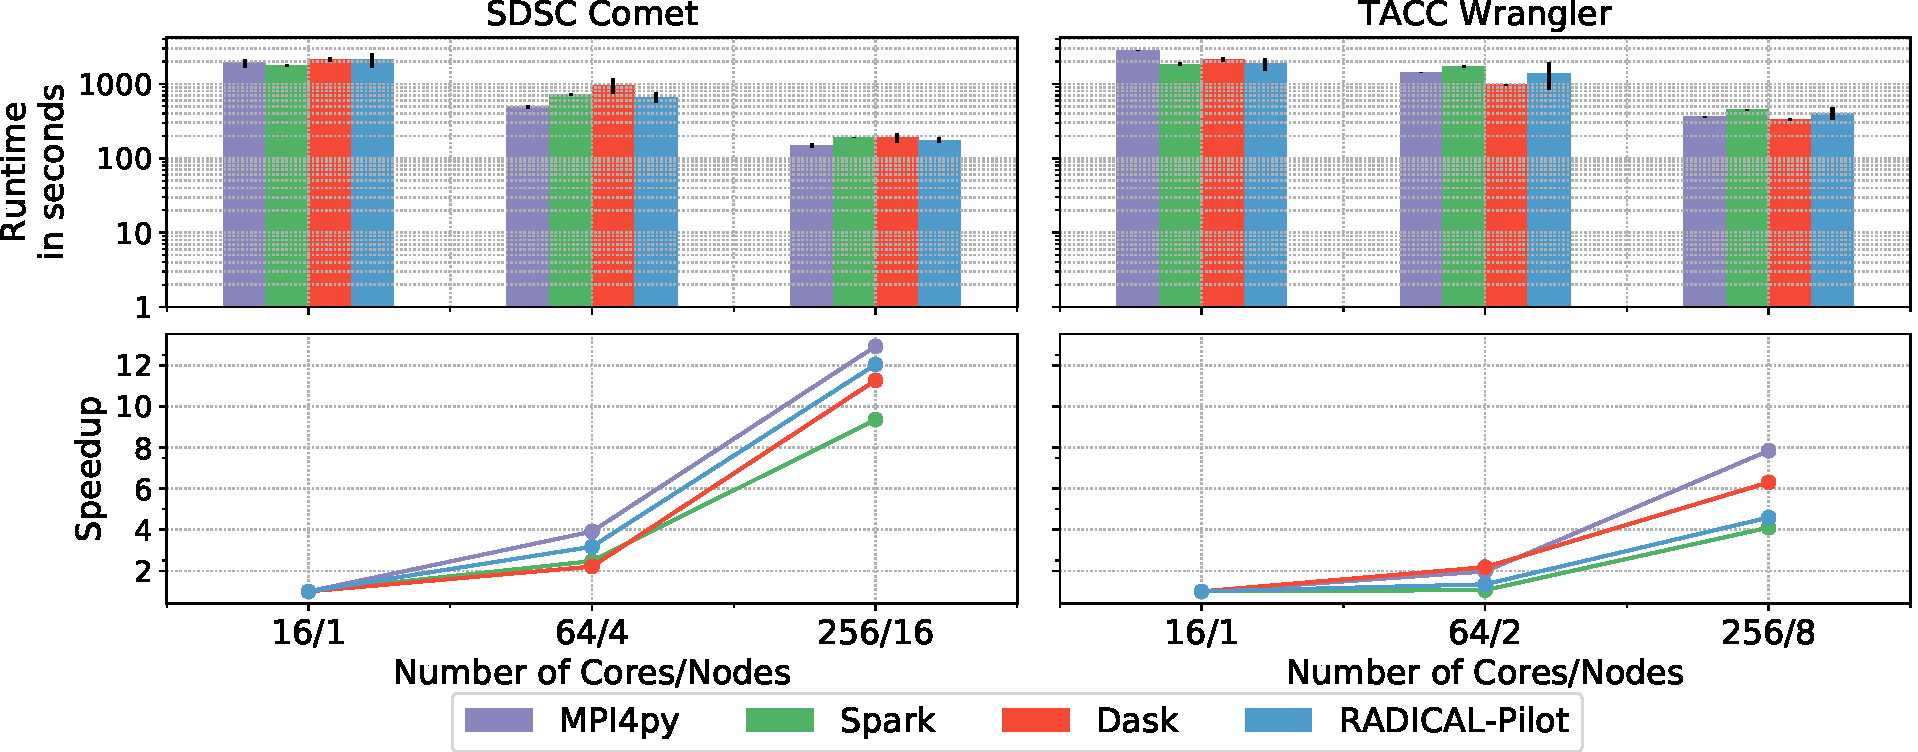
\includegraphics[width=.95\textwidth]{figures/data_analytics_hpc/task_par/comet_wrangler_haus.pdf}
    \caption{Time to completion and speedup of Hausdorff Distance execution on Comet and Wrangler for 128 large trajectories.} 
    \label{fig:comet_wrangler_haus}
\end{figure}

MPI4py, RADICAL~-Pilot, Spark and Dask have similar performance when used to execute embarrassingly parallel algorithms.
All frameworks achieved similar speedups as the number of cores increased, scaling by a factor of 6 from 16 to 256 cores, which are lower than MPI4py.
Although, the frameworks' overheads are comparably low in relation to the overall runtime, they were significant to impact their speedup.
RADICAL~-Pilot's large deviation is due to sensitivity to communication delays with the database.
In summary, all three frameworks provide appropriate abstractions and runtime performance, compared to MPI, for embarrassingly parallel algorithms. 
In this case aspects such as programmability and integrate-ability are more important considerations,e.\,g., both RADICAL~-Pilot and Dask are native Python frameworks making the integration with python native frameworks easier and more efficient than with other frameworks, which are based on other languages.

%\begin{figure}[ht]
%    \centering
%    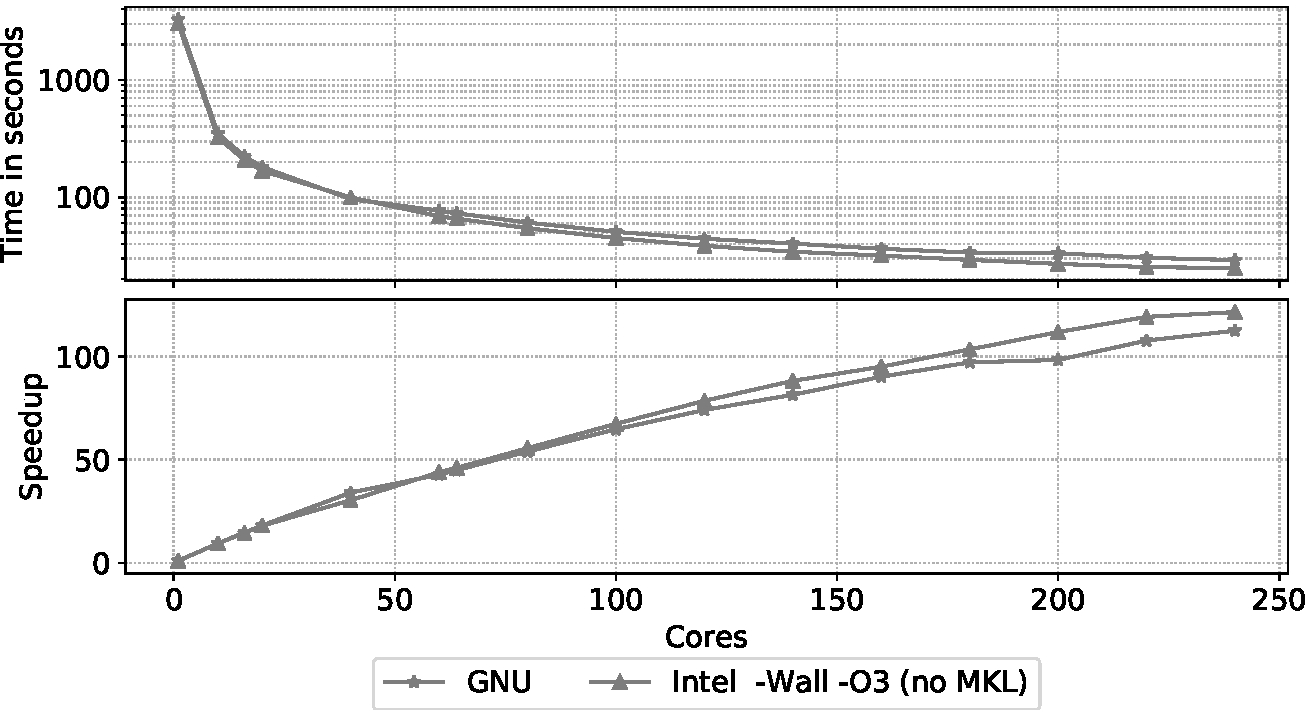
\includegraphics[width=.95\textwidth]{figures/data_analytics_hpc/task_par/cpptrajHausdorff.pdf}
%    \caption{\label{fig:cpptraj_resutls}\textbf{Hausdorff Distance using CPPTraj:}
%    Runtimes and Speedup over different number of cores.} 
%\end{figure}

%CPPTraj~\cite{roe2018parallelization} provides an optimized C++ implementation of the 2D-RMSD, which is Algorithm~\ref{alg:hausdorff} with no $\min-\max$ operations.
%The 2D-RMSD between trajectories was executed in parallel.
%The results were gathered and the Hausdorff distance was calculated.
%CPPTraj~\cite{roe2018parallelization} was compiled with GNU C++ compiler and no optimizations, and with Intel's compiler O3 optimization enabled.
%An experiment was run with 20-core Haswell nodes and 128 small trajectories; number of cores ranging from 1 up to 240.
%Figure~\ref{fig:cpptraj_resutls} shows the runtimes and speedup.
%MPI C++ provides lower execution times.
%However, we are interested in scalable solutions, that may offer worse performance in absolute numbers, but allows easier integration, i.e., less lines of code, and/or less engineering time.

\subsection{Leaflet Finder}
\label{sec:leaflet}
\begin{table*}[t]
    \centering
    \begin{tabular}{@{}p{2cm}|p{2.8cm}p{2.8cm}p{2.8cm}p{2.8cm}@{}}
        \toprule
        &
        \textbf{Broadcast and 1-D} (Approach 1) &
        \textbf{Task API and 2-D} (Approach 2) &
        \textbf{Parallel Connected Components} (Approach 3) &
        \textbf{Tree-Search} (Approach 4)\\
        \midrule
        % row 1
        Data Partitioning  & 
        1D  & 
        2D & 
        2D & 
        2D\\
        % row 2
        Map & 
        Edge Discovery via Pairwise Distance &
        Edge Discovery via Pairwise Distance &
        Edge Discovery via Pairwise Distance and Partial Connected Components & 
        Edge Discovery via Tree-based Algorithm and Partial Connected Components\\
        % row 3
        Shuffle &
        Edge List ($O(E)$) &
        Edge List ($O(E)$) &
        Partial Connected components ($O(n)$) &
        Partial Connected components ($O(n)$)\\
        % row 4
        Reduce   &
        Connect Components  &
        Connected Components &
        Joined Connected Components &
        Joined Connected Components\\
        \bottomrule
    \end{tabular}
    \caption{MapReduce Operations used by Leaflet Finder\label{tab:app_operators}}
\end{table*}

\begin{figure*}[t]
    \centering
    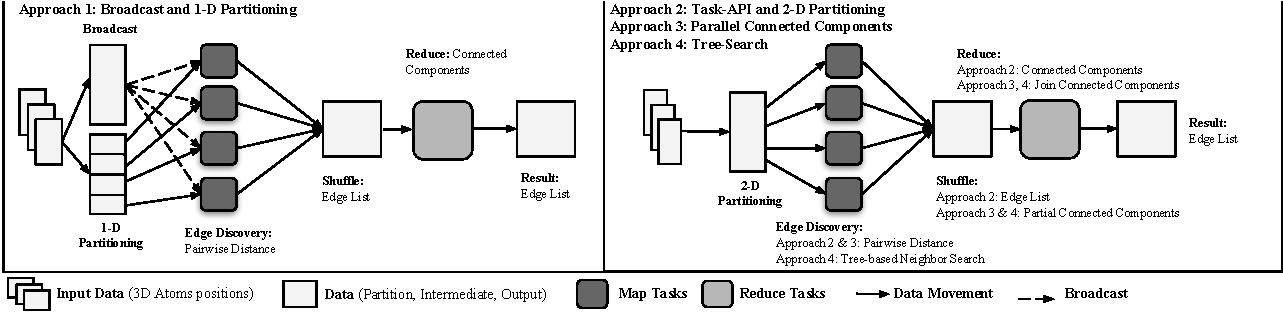
\includegraphics[width=.98\textwidth]{figures/data_analytics_hpc/task_par/lf_approaches.pdf}
    \caption{Architectural approaches for implementing the Leaflet finder algorithm\label{fig:lf_approaches}} 
\end{figure*}

We developed four different approaches for implementing the Leaflet Finder algorithm using RADICAL~-Pilot, Spark, Dask, and MPI4py (see Fig~\ref{fig:lf_approaches} and Table~\ref{tab:app_operators}):
\begin{enumerate}[1)]
    \item \textbf{Broadcast and 1-D Partitioning:}
    The physical system is broadcast and partitioned through a data abstraction.
    Use of RDD API (broadcast), Dask Bag API (scatter), and MPI Bcast to distribute data to all nodes.
    A \texttt{map} function calculates the edge list using \texttt{cdist} from SciPy~\cite{scipy} -- realized as a loop for MPI.
    The list is collected to the master process (gathered to rank 0) and the connected components are calculated.\label{en:1}
    \item \textbf{Task API and 2-D Partitioning:}
    Data management is done without using the data-parallel API.
    The framework is used for task scheduling.
    Data are pre-partitioned in 2-D partitions and passed to a \texttt{map} function that calculates the edge list using \texttt{cdist}-- realized as a loop for MPI.
    The list is collected (gathered to rank 0) and the connected components are calculated.\label{en:2}
    \item \textbf{Parallel Connected Components:}
    Data are managed as in approach~\ref{en:2}.
    Each \texttt{map} task performs edge list and connected components computations.
    The reduce phase joins the calculated components into one, when there is at least one common node.\label{en:3}
    \item \textbf{Tree-based Nearest Neighbor and Parallel-Connected Components (Tree-Search):}
    This approach is different to approach~\ref{en:3} only on the way edge discovery in the \texttt{map} phase is implemented.
    A tree containing all atoms is created which is then used to query for adjacent atoms.\label{en:4}
\end{enumerate}

We use four physical systems with $131k$, $262k$, $524k$, and $4M$ atoms with $896k$, $1.75M$, $3.52M$, and $44.6M$ edges in their graphs.
Experimentation was conducted on Wrangler where we utilized up to 256 cores.
Data partitioning results into $1024$ partitions for each approach, thus $1024$ \texttt{map} tasks.
Due to memory limitations from using \texttt{cdist} -- uses double precision floating point -- Approach \ref{en:3} data partitioning of the $4M$ atom dataset resulted to $42k$ tasks for both Spark and MPI4py.

Figure \ref{fig:All4approachesNoRp} shows the runtimes for all datasets for Spark, Dask and MPI4py.
RADICAL~-Pilot's performance is illustrated in Figure~\ref{fig:rpLF}.
We continue by analyzing the performance of each architectural approach and used framework in detail.

\begin{figure}[t]
    \begin{subfigure}{.95\textwidth}
        \centering
        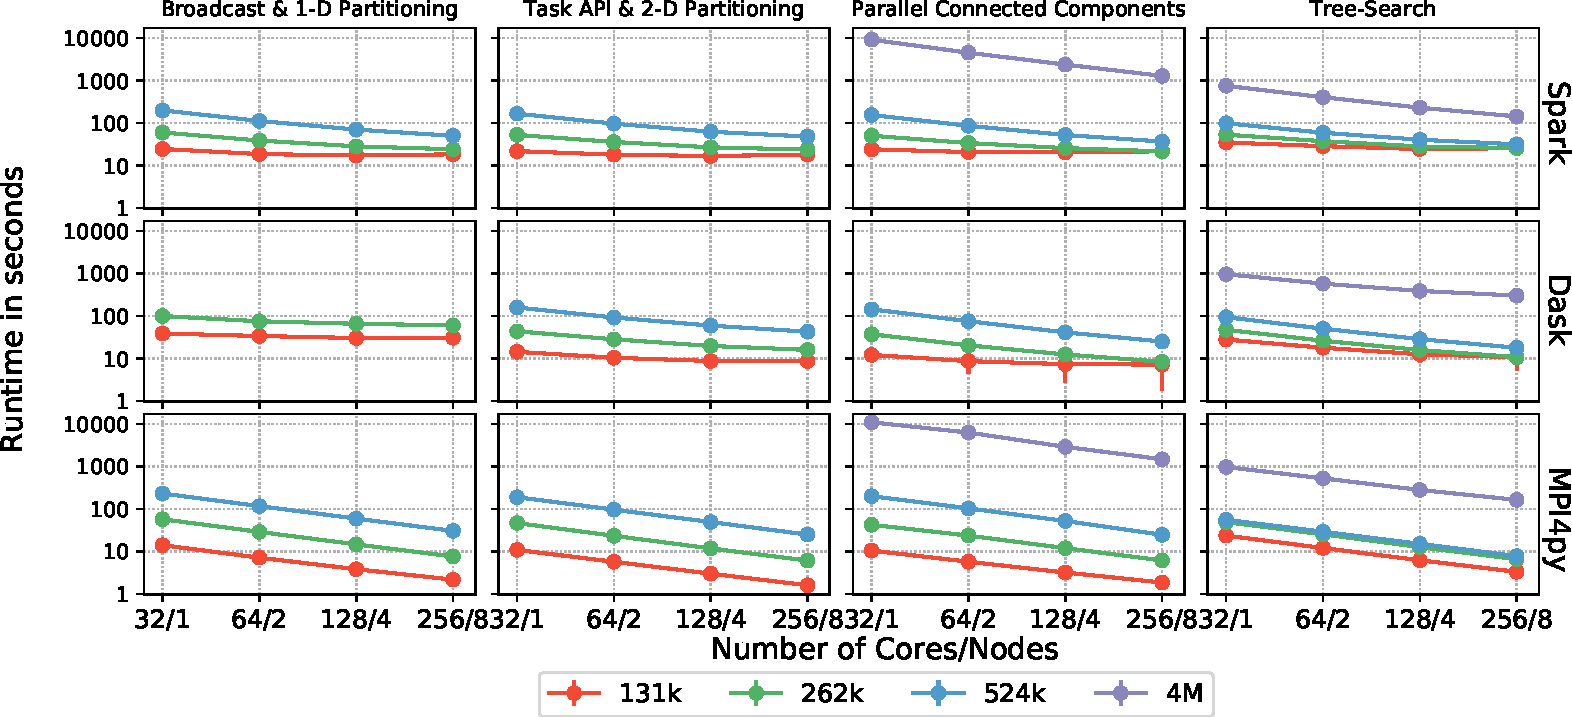
\includegraphics[width=1\linewidth]{figures/data_analytics_hpc/task_par/All4approachesWith4M_logscaleline.pdf}
    \end{subfigure}\\
    \begin{subfigure}{.95\textwidth}
        \centering
        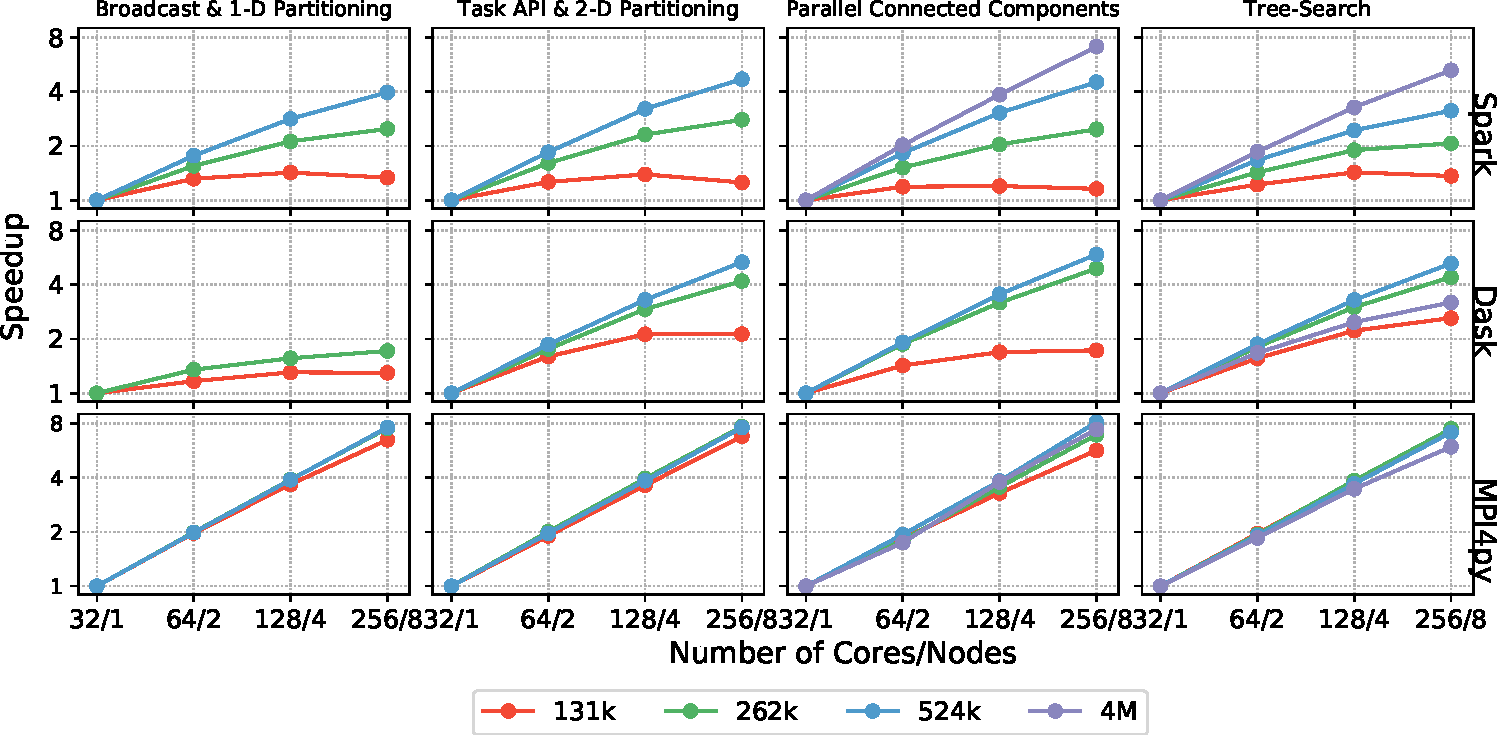
\includegraphics[width=.95\linewidth]{figures/data_analytics_hpc/task_par/All4approachesWith4MSpeedup.pdf}
    \end{subfigure}
    \caption{Leaflet Finder Performance of Different Architectural Approaches for Spark \& Dask.
            Runtimes and Speedups for different system sizes over different number of cores for all approaches and frameworks.}
    \label{fig:All4approachesNoRp}
\end{figure}

%%%%%%%%%%%%%%% APPROACH 1 %%%%%%%%%%%%%%%%%%

\begin{figure}[t]
    \centering
    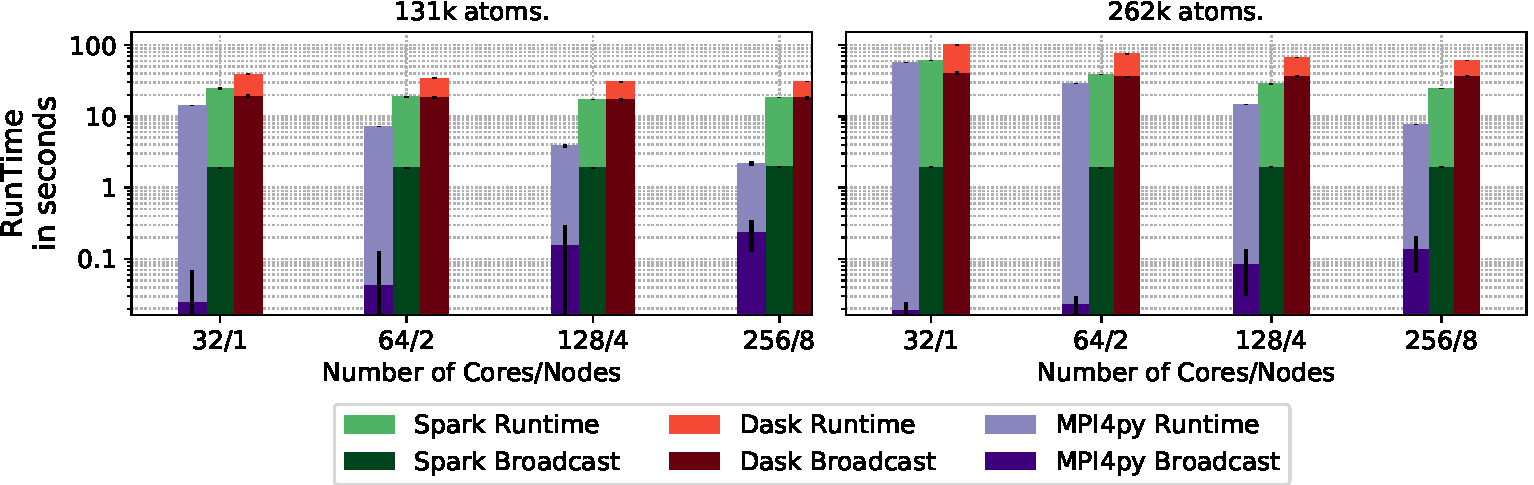
\includegraphics[width=.95\textwidth]{figures/data_analytics_hpc/task_par/spark_dask_lf_approach1.pdf}
    \caption{Broadcast and 1-D Partitioned Leaflet Finder (Approach 1).
    Runtime for multiple system sizes on different number of cores for Spark, Dask and MPI4py.}
    \label{fig:WranglerLeafLetFinderApp1}
\end{figure}

\subsubsection*{Broadcast and 1-D Partitioning}
Approach 1 utilizes a broadcast to distribute the data to all nodes, which is supported by Spark, Dask and MPI.
All nodes maintain a complete copy of the dataset.
Each \texttt{map} task computes the pairwise distance on its partition.
We use 1-D partitioning.
Figure~\ref{fig:WranglerLeafLetFinderApp1} shows the detailed results: as expected the usage of a broadcast has severe limitations for Spark and Dask.
MPI broadcast is a fraction of the overall execution time and significantly smaller than Spark and Dask.
MPI's broadcast times increase linearly as the number of processes increases, while Spark's and Dask's remain relatively constant for each dataset, due to more elaborate broadcast algorithms compared to MPI.
Broadcast times are about $3\%$ -- $15\%$ of the edge discovery time for Spark, $40\%$ -- $65\%$ for Dask, and $<1\%$ -- $10\%$ for MPI4py.
Spark offers a more efficient communication subsystem compared to Dask.
In addition, Dask broadcast partitions the dataset to a list where each element represents a value from the initial dataset.
This did not allow broadcasting the $524k$ atom dataset.
Nevertheless, the limited scalability of this approach due to transmitting the entire dataset renders it only usable for small datasets.
It shows the worst performance and scaling of all approaches for Spark, Dask and MPI4py.

Furthermore, this approach only scales up to $262k$ atoms for Dask, and $524k$ atoms for Spark and MPI4py on Wrangler.
Spark's performance is comparable to MPI4py for the $262k$, and $524k$ datasets.
It also shows better performance for the smallest core count in the $524k$ case.
Dask is at least two times slower than our MPI implementation.

%%%%%%%%%%%%%%% APPROACH 2 %%%%%%%%%%%%%%%%%%


\begin{figure}[t]
    \centering
    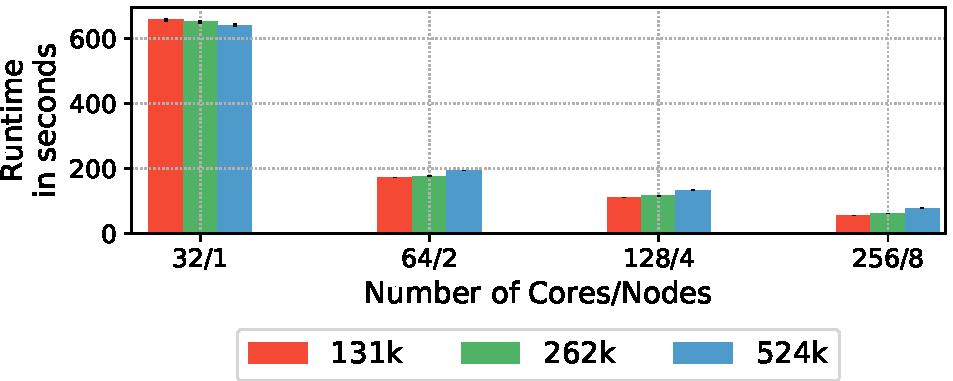
\includegraphics[width=.95\textwidth]{figures/data_analytics_hpc/task_par/rpLF.pdf}
    \caption{RADICAL~-Pilot Task API and 2-D Partitioned Leaflet Finder (Approach 2).
    Runtime for multiple system sizes over different number of cores.}
    %Overheads dominate since execution times are similar despite the system size.}
    \label{fig:rpLF}
\end{figure}

\subsubsection*{Task-API and 2-D Partitioning}
Approach~\ref{en:2} tries to overcome the limitations of approach 1, especially broadcasting and 1-D partitioning.
A 2-D block partitioning is essential, as it evenly distributes the compute and more efficiently utilizes the available memory.
2-D partitioning is not well supported by Spark and Dask.
Spark's RDDs are optimized for data-parallel applications with 1-D partitioning.
While Dask's array supports 2-D block partitioning, it was not used for this implementation.
We return the adjacency list of the graph instead of an array to fully use the capabilities of the abstraction.
Thus, each task works on a 2-D pre-partitioned part of the input data.

Figure~\ref{fig:All4approachesNoRp} shows the runtimes of approach~\ref{en:2} for Spark, Dask, MPI4py and Figure~\ref{fig:rpLF} for RADICAL~-Pilot.
As expected this approach overcomes the limitations of approach 1 and can easily scale to larger datasets (e.\,g., $524k$ atoms) while improving the overall runtime.
Dask's execution time was smaller by at least a factor of two.
However, we were not able to scale this implementation to the 4M dataset, due to memory requirements of \texttt{cdist}.
For RADICAL~-Pilot we observed significant task management overheads (see also section~\ref{sec:framework_eval}).
This is a limitation of RADICAL~-Pilot with respect to managing large numbers of tasks.
This is particularly visible when the scenario was run on a single node with 32 cores.
As more resources become available, i.e. more than 64 cores, the performance improves dramatically.

Furthermore, Spark and Dask did not scale as well as MPI, which achieved linear speedups of $\sim8$ when using $256$ cores.
Spark and Dask achieved maximum speedups of $4.5$ and $\sim5$ respectively.
Despite this fact, both frameworks had similar performance on $32$ cores for the $262k$ and $524k$ datasets.

%%%%%%%%%%%%%% Approach 3 %%%%%%%%%%%%%%%%%%%%%%%

\subsubsection*{Parallel Connected Components}
Communication between the edge discovery and connected components stages is another important aspect.
The edge discovery phase output for the $524k$ atoms dataset is $\approx$ $100\,\textup{MB}$.
To reduce the amount of data that need to be shuffled, we refined the algorithm to compute the graph components on the partial dataset in the \texttt{map} phase.
The partial components are then merged in a \texttt{reduce} phase.
This reduces the amount of shuffle data by more than $50\%$ (e.\,g., to $12\textup{MB}$ for Spark and $48\textup{MB}$ for Dask).
Figure~\ref{fig:All4approachesNoRp} shows the improvements in runtime, by $\sim20\%$ for Spark and Dask, but not MPI4py.
Further, we were able to run very large datasets, such as the 4M dataset, using this architectural approach using Spark and MPI4py.
Dask was restarting its worker processes because their memory utilization was reaching $95\%$.

Spark, and Dask have comparable performance with MPI on 32 cores, which utilizes a single node on Wrangler.
However, the MPI4py implementation scales almost linearly for all datasets, Spark and Dask cannot, reaching a maximum of $\sim5$ for the three smaller datasets.
In addition, Spark is able to scale almost linearly for the $4M$ atoms dataset providing comparable performance to MPI4py.

%%%%%%%%%%%%%% Approach 4 %%%%%%%%%%%%%%%%%%%%%%%

\subsubsection*{Tree-Search}
A bottleneck of approaches~\ref{en:1},~\ref{en:2} and~\ref{en:3} is the edge 
discovery via the naive calculation of the distances between all pairs of atoms. 
In approach~\ref{en:4}, we replace the pairwise distance function with a tree-based, 
nearest neighbor search algorithm, in particular BallTree~\cite{omohundro89five}. 
The algorithm: 
\begin{inparaenum}
    \item constructs of a tree, and
    \item queries for neighboring atoms.
\end{inparaenum}

Using tree-search, the computational complexity can be reduced from $n^2$ to $log$. 
We use a BallTree as offered by Scikit-Learn~\cite{scikit-nearest} for our implementation.

Figure \ref{fig:All4approachesNoRp} illustrates the performance of the implementation.
For small datasets, i.\,e., $131k$ and $262k$ atoms, approach~\ref{en:3} is faster than the tree-based approach, since the number of points is too small.
For the large datasets, the tree approach is faster.
In addition, the tree has a smaller memory footprint than \texttt{cdist}.
This allowed to scale to larger problems, e.\,g., a $4M$ atoms and $44.6M$ edges dataset without changing the total number of tasks.

Dask shows better scaling than Spark for $131k$, $262k$, and $524k$ atoms.
This is not true for $4M$ atoms, indicating that Dask's communication layer is not able to scale as well as Spark's.
Spark shows similar performance with MPI4py for the largest dataset due to minimal shuffle traffic.
Thus, MPI's efficient communication does not become relevant.

\section{Task-Parallel Framework Selection Conceptual Model and Discussion}
In this section we provide a conceptual model that allows application developers to carefully select a framework according to their requirements (e.\,g., compute and I/O).
It is important to understand both the properties of the application and Big Data frameworks.
Table~\ref{tab:framework} illustrates the criteria of this conceptual model and ranks the three frameworks.

\begin{table}[t]
    \centering
    \begin{tabular}{@{}cccc@{}}
        \toprule
        &\textbf{RADICAL~-Pilot}     &\textbf{Spark} &\textbf{Dask}\\
        \multicolumn{4}{l}{\textbf{Task Management}} \\
        \midrule
        Low Latency   &- &o &+\\
        Throughput    &- &+ &++\\
        MPI/HPC Tasks &+ &o &o\\
        Task API   &+ &o &++\\
        Large Number of Tasks   &-- &++ &++\\\hline
        \multicolumn{4}{l}{\textbf{Application Characteristics}}\\\midrule
        Python/native Code &++ &o &+\\
        Java               &o &++ &o\\
        Higher-Level Abstraction &- &++ &+\\
        Shuffle                  &- &++ &+\\
        Broadcast                &- &++ &+\\
        Caching                  &- &++ &o\\
        \bottomrule
    \end{tabular}
    \caption{Task-parallel framework selection decision methodology: Criteria and Ranking for Framework Selection. -~: Unsupported or low performance
        +~: Supported, ++~: Major Support, and o~:Minor support.\label{tab:framework}}
\end{table}
%  application perspective

\subsubsection*{Application Perspective}
We showed that we can implement MD trajectory data analysis applications using all three frameworks, as well as MPI4py.
Implementation aspects, such as computational complexity, and shuffled data size influence the performance greatly.
For embarrassingly parallel applications with coarse grained tasks, such as PSA, the choice of the framework does not significantly influence performance (Figures~\ref{fig:HausdorffWrangler} and~\ref{fig:comet_wrangler_haus}).
In addition, the performance difference against MPI4py was not significant (Figures~\ref{fig:HausdorffWrangler} and~\ref{fig:comet_wrangler_haus}).
Thus, aspects, such as programmability and integrate-ability, become more important.

For fine-grained data parallelism, a Big Data framework, such as Spark and Dask, clearly outperforms RADICAL~-Pilot (Figures~\ref{fig:All4approachesNoRp},~\ref{fig:rpLF}).
If coupling is introduced, i.\,e. task communication is required (e.\,g., reduce), using Spark becomes advantageous (Approaches~\ref{en:3} \& \ref{en:4}). 
PI4py outperformed Dask, and Spark, despite both frameworks scaling for the larger datasets.
Especially Spark was able to provide linear speedup for approach~\ref{en:3} of Leaflet Finder (Figure~\ref{fig:All4approachesNoRp}).
Integrating with frameworks that provide higher level abstractions provides scalable solutions for more complex algorithms.
However, integrating Spark with other tools needs to be carefully considered.
The integration of Python tools, e.\,g. MDAnalysis, often causes overheads due to the frequent need for serialization and copying data between the Python and Java space.

Dask had the smallest learning curve of all three frameworks.
As a result, it allows for faster prototyping compared to RADICAL~-Pilot and Spark.
RADICAL~-Pilot's learning curve is more steep, but is more versatile than Dask and Spark, by offering the lowest level abstraction. 
Spark had the slowest learning curve.
It required tuning to get the number of tasks correctly, as well as argument passing to map and reduce functions.

\subsubsection*{Framework Perspective}
RADICAL~-Pilot is well suited for HPC applications, e.\,g., ensembles (up to $50k$ tasks) of parallel MPI applications, as shown in Ref.~\cite{merzky2018design,merzky2019using}.
It has limited scalability when supporting large numbers of short-running tasks, as often found in data-intensive workloads.
The file staging implementation of RADICAL~-Pilot is not suitable for supporting the data exchange patterns, i.e. shuffling, required for these applications.
However, executing MPI and Spark applications alongside on the same resource makes RADICAL~-Pilot particularly suitable when different programming models need to be combined.

% framework perspective
Dask provides a highly flexible, low-latency task management and excellent support for parallelizing Python libraries.
We established that Dask has higher throughput (Figures~\ref{fig:dask_spark_rp_wrangler} and~\ref{fig:RP_Dask_Spark_throughput}).
However, Spark provides better speedups for the largest datasets compared to Dask (Figure ~\ref{fig:All4approachesNoRp}).
Dask's broadcast (Leaflet Finder approach~\ref{en:1}) and shuffle (Leaflet Finder approaches~\ref{en:2}-~\ref{en:4}) performance is worse for larger problems compared to Spark.
Thus, Dask's communication layer shows some weaknesses that are particularly visible during broadcast and shuffle.
Spark needs to be particularly considered for shuffle-intensive applications.
Its in-memory caching mechanism is particularly suited for iterative algorithms that maintain a static set of data in-memory and conduct multiple passes on that set.
